\textbf{COLUNI 2025 -- Questão 31}\par\medskip As alterações nos padrões de clima e de temperatura causadas pelo homem direta ou indiretamente são chamadas de mudanças climáticas. As mudanças climáticas não só englobam o aquecimento global, que é o aumento da temperatura média superficial do planeta Terra, mas também todas as consequências que derivam dele, como as secas frequentes, os incêndios florestais, o derretimento das calotas polares, as tempestades catastróficas, a escassez de água e o aumento do nível do mar.

\noindent Disponível em: https://www.unicef.org/brazil/blog/os-desastres-brasileiros-e-suas-relacoes-com-mudancas-climaticas. Acesso em: 25 mai.2024.

\par

Em maio de 2024, o estado do Rio Grande do Sul sofreu uma das maiores tragédias de sua história. Chuvas constantes e intensas contribuíram para grandes enchentes em diversos municípios gaúchos, expulsando uma grande quantidade de pessoas e animais e destruindo muitas cidades.

\begin{center}Chuvas causam inundações e destruição no Rio Grande do Sul.\end{center}

\noindent\begin{minipage}[t]{0.48\linewidth}\centering
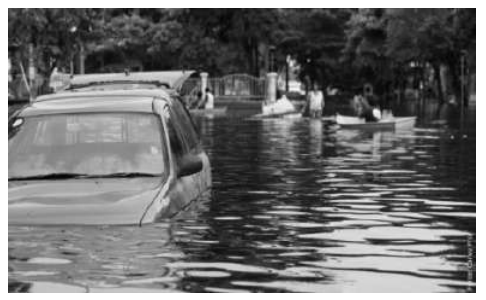
\includegraphics[width=\linewidth]{static/simulados/coluni/figuras/2025/questao-31/figura-1.png}
\end{minipage}\hfill\begin{minipage}[t]{0.48\linewidth}\centering
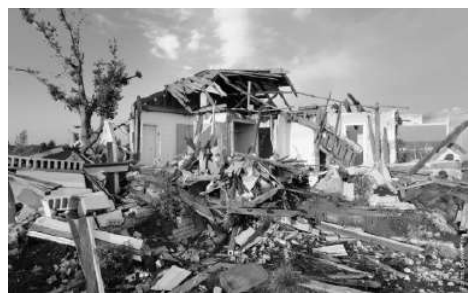
\includegraphics[width=\linewidth]{static/simulados/coluni/figuras/2025/questao-31/figura-2.png}
\end{minipage}

\begin{center}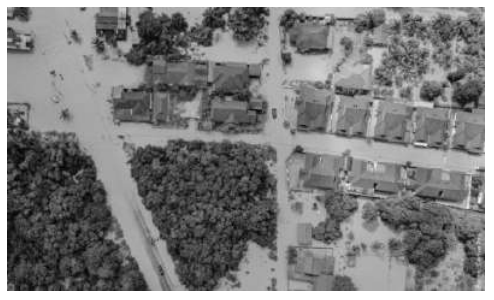
\includegraphics[width=0.42\linewidth]{static/simulados/coluni/figuras/2025/questao-31/figura-3.png}\end{center}

\noindent Disponível em: https://aguasustentavel.org.br/conteudo/blog/242-enchentes-devastadoras-rs. Acesso em: 22 mai. 2024.

\par

Considerando o fenômeno ilustrado, é CORRETO afirmar que:
\begin{enumerate}
\item trata-se de um evento climático extremo, provocado por um fator preponderante, a presença de uma frente fria, que reduziu drasticamente a temperatura antecipando a chegada do inverno.
\item as intensas chuvas são comuns na região, principalmente, na área metropolitana de Porto Alegre onde a elevada concentração populacional contribui com o desmatamento e assoreamento dos rios locais.
\item o uso intensivo da agropecuária gaúcha, uma das mais importantes do Brasil, contribuiu para a ocorrência de enchentes e transbordamento dos rios devido ao intenso processo erosivo que ocorre em suas margens.
\item é o resultado do intenso uso das bacias hidrográficas dos rios Taquari, Caí e Guaíba, importantes no sistema de drenagem que, ao chegarem na Lagoa dos Patos, não tiveram vazão suficiente para evitar as inundações.
\end{enumerate}
